\documentclass[12pt, a4paper]{article}
\usepackage{amsmath}
\usepackage{amsfonts}
\usepackage{amsthm}
\usepackage{mathtools}
\newtheorem{theorem}{Theorem}[section]
\newtheorem{definition}{Definition}[section]
\numberwithin{equation}{section}
\usepackage{pgfplots}
\pgfplotsset{width=10cm,compat=1.9}

\title{Information theory}
\author{Kristian Wichmann}

\begin{document}
\maketitle

\section{Self-information or surprisal}
Let $X$ be a random variable. Consider an event $A$. We may ask ourselves how much information $I(A)$ - also known as \textit{self-information} or \textit{surprisal} - we have gained by having this event occuring. It is clear, that such a quantity must depend only on the probability of the event:
\begin{equation}
I(A)=I(P(A))
\end{equation}
Therefore, we can express self-information through a function $f(p)$, so that if $P(A)=p$, then $I(A)=f(p)$.

If the outcome of an event $A$ is certain, i.e. if $P(A)=1$ then we have gained no information. So we must have $P(A)=1\Rightarrow I(A)=0$. or in other words $f(1)=0$. Non-certain events occuring, on the other hand, should give us non-zero information. So for $p<1$ we should have $f(p)>0$.

Further, if two events $A$ and $B$ are independent it seems reasonable to require that self-information is additive is the following sense:
\begin{equation}
\label{self_information_additivity}
I(A\cap B)=I(A)+I(B)
\end{equation}
So if two independent events happen at the same time, self-information should simply add up. Because of independence, we also have:
\begin{equation}
P(A\cap B)=P(A)\cdot P(B)
\end{equation}
Applying $f$ to both sides of this equation we get:
\begin{equation}
I(A\cap B)=f(P(A)\cdot P(B))
\end{equation}
Combine this with equation $(\ref{self_information_additivity})$ to get:
\begin{equation}
f(P(A)\cdot P(B))=f(P(A))+f(P(B))
\end{equation}
The only functions having this property are logarithms. Hence, the self-information must be of the form:
\begin{equation}
f(p)=-k\cdot\log(p)
\end{equation}
The minus sign comes from requiring $f(p)>0$ for $p<1$. This means that $k$ will be positive, but apart from that can be chosen freely. Since all logarithms are proportional to each other, this is equivalent to choice of base $b$ being free:
\begin{equation}
f(p)=-\log_b(p)
\end{equation}

\subsection{Continous distributions?}
The section above deals with discrete random variables? However, we run into problems if we try to mindlessly generalize to continous variables: The "obvious" analogue of the self-information for the outcome $X=x$ the would be $-\log_b f(x)$, where $f(x)$ is the probablity density function of $X$. But since this function need not be below 1, the associated surprisal is actually negative! Clearly, something is fishy. But for now, we will only consider discrete random variables.

\section{Entropy}
The \textit{entropy} of a discrete random variable $X$ is the expectation value of the self-information:
\begin{equation}
H(X)=E[I(X)]=E[-\log_b(X)]
\end{equation}
Here, $I(X)$ is itself a stochastic variable. Thus, entropy can be interpreted as the expected surprisal. Since $X$ is discrete, we may write:
\begin{equation}
H(X)=-\sum_x p(x)\log_b p(x)
\end{equation}
Figure $\ref{fig:entropy_graph}$ shows how much an outcome of $p$ contributes to the total entropy. Since the limit for $p\rightarrow 0$ tends to zero, we will extend the definition to outcomes with zero probability; these do not contribute to the entropy.

\begin{figure}
\centering
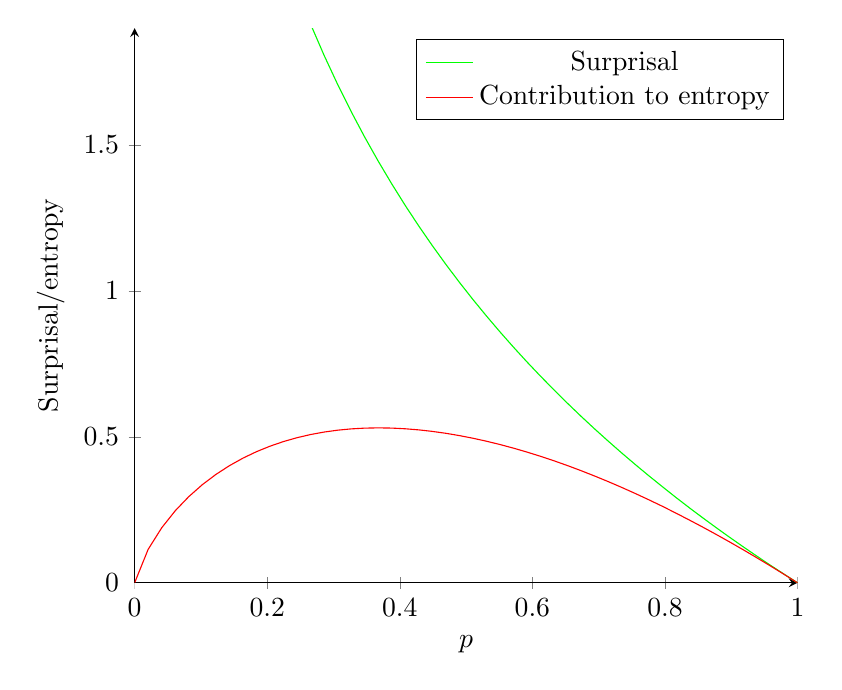
\begin{tikzpicture}
\begin{axis}[
    axis lines = left,
    xlabel = $p$,
    ylabel = {Surprisal/entropy},
    ymin = 0,
    ymax = 1.9,
]
\addplot [
    domain=0:1, 
    samples=50, 
    color=green,
]
{-ln(x)/ln(2)};
\addlegendentry{Surprisal}

\addplot [
    domain=0:1, 
    samples=50, 
    color=red,
]
{-x*ln(x)/ln(2)};
\addlegendentry{Contribution to entropy}
\end{axis}
\end{tikzpicture}
\caption{Surprisal and contribution to entropy as a function of $p$. Here for $b=2$.}
\label{fig:entropy_graph}
\end{figure}

\subsection{Different choices of $b$}
As mentioned above, we're free to choose $b$, but some choices are common. Each carry its own unit of entropy with it:
\begin{itemize}
\item $b=2$: The corresponding entropy is known as \textit{Shannon entropy}, and the unit is Shannon or simply bits.
\item $b=e$: The corresponding unit is known as a nat.
\item $b=10$: The corresponding unit is known as a Hartley.
\end{itemize}
Unless explicitly mentioned, we will use Shannon entropy from now on.

\end{document}